\chapter{Supplementary Texts}
\label{appendix:background:supplementary_texts}

\section{Background}
\label{sec:appendix:texts:background}

\subsection{Levels of Autonomy}
\label{subsec:appendix:texts:background:levels_of_autonomy}
\begin{itemize}
	\item \textbf{Level 0 ("'Active driver"'):} No computer assistance of any kind. A car is completely controlled by its human driver.
	\item \textbf{Level 1 ("'Feet off"'):} Basic assistance, e.g. adaptive cruise control. While most functions are controlled by the driver, the car might take responsibility of a single task, e.g. accelerating and decelerating in certain scenarios.
	\item \textbf{Level 2 ("'Hands off"'):} Partial automation, e.g. cruise control and lane centering. At this level, a car is able to take over multiple driving tasks in combination. While the driver is still required to monitor the roadway, she is "'disengaged from physically operating the vehicle"' \cite{Klein} and may keep her hands of the steering wheel and feet of the pedals. To ensure that a driver is still pays full attention and is able to intervene in case of system failures or critical situations, various methods of \textit{Driver Monitoring} are employed. Such include to visually observe a driver's face using cameras or to measure the force applied to the steering wheel.
	\item \textbf{Level 3 ("'Eyes off"'):} High degree of automation. At this level, a driver might fully rely on a car's self-driving under most conditions, delegating all safety-critical function to the ADAS. Usually, it would maintain a comprehensive awareness of its environment and is able to react on it. Although a driver still has to be present and prepared to take occasional control, she is not required to constantly monitor the traffic. 
	\item \textbf{Level 4 ("'Attention off"'):} Full automation. This refers to a system that is able to "'perform all safety-critical driving functions and monitor roadway conditions for an entire trip."' \cite{2016transportation} At this level, there is no necessity for a driver to actually occupy the vehicle.Driving performance of Level 4 autonomous cars is at least equal to human level and would generally even surpass it. 
	\item \textbf{Level 5 ("'Passive passenger"'):} Full autonomy. The highest level of automation describes a system that is capable of driving under any conditions, even extreme ones. Its performance is expected to be at least human-like or even surpass human driving capabilities. 
\end{itemize}

With this classification, it is worth noting that only the highest level actually refers to the term "'autonomy"'. \cite{wood2012potential} states that although this term is in more widespread public use, speaking of "'automation"' would be more accurate for levels 1 to 4. Only Level 5 cars are self-governing and may take independent decisions, e.g. selecting a destination and an appropriate route, while cars of all other levels still have a human person in the driver's seat.

\section{Related Work}
\label{sec:appendix:texts:related_work}

\subsection{Further Modeling and Representation Approaches}
\label{subsec:appendix:texts:related_work:state_represtation}
Another standard exists with \textbf{DATEX II}, specified by the European Committee for Standardization \cite{Dolger2011}. The XML-based format is meant for \textit{"'exchanging traffic information between traffic management centres, traffic service providers, traffic operators and media partners"'} \cite{wiki:datex2}, however, not particularly for cooperative perception. It defines a way to describe traffic events, such as road works or congestions as well as information on the current parking situation. However, it is not suitable to describe particular traffic situations in high detail. the same holds true for the \textbf{SENSORIS} representation format presented by \cite{Hohm2019}, that was designed in a different way, but with the same purpose.
\par
\medskip

\cite{Stiller2012} follows yet a different approach as the authors show a way to represent the current local world state as the instantiation of a \textbf{Markov Logic Network}, in which weights represent uncertainty about the true state of an observation. This representation is inherently graphical and by incorporating first-order logic, the underlying model also allows for basic inference, in theory. A specification of what objects and relations to include to comprehensively model a traffic scene is not provided.

\section{Concept \& Design}
\label{sec:appendix:texts:concept_design}

\subsection{Geographical Sharding Schema}
\label{subsec:appendix:texts:concept_design:geographical_partitioning_schema}
\begin{figure}[H]
	\centering
	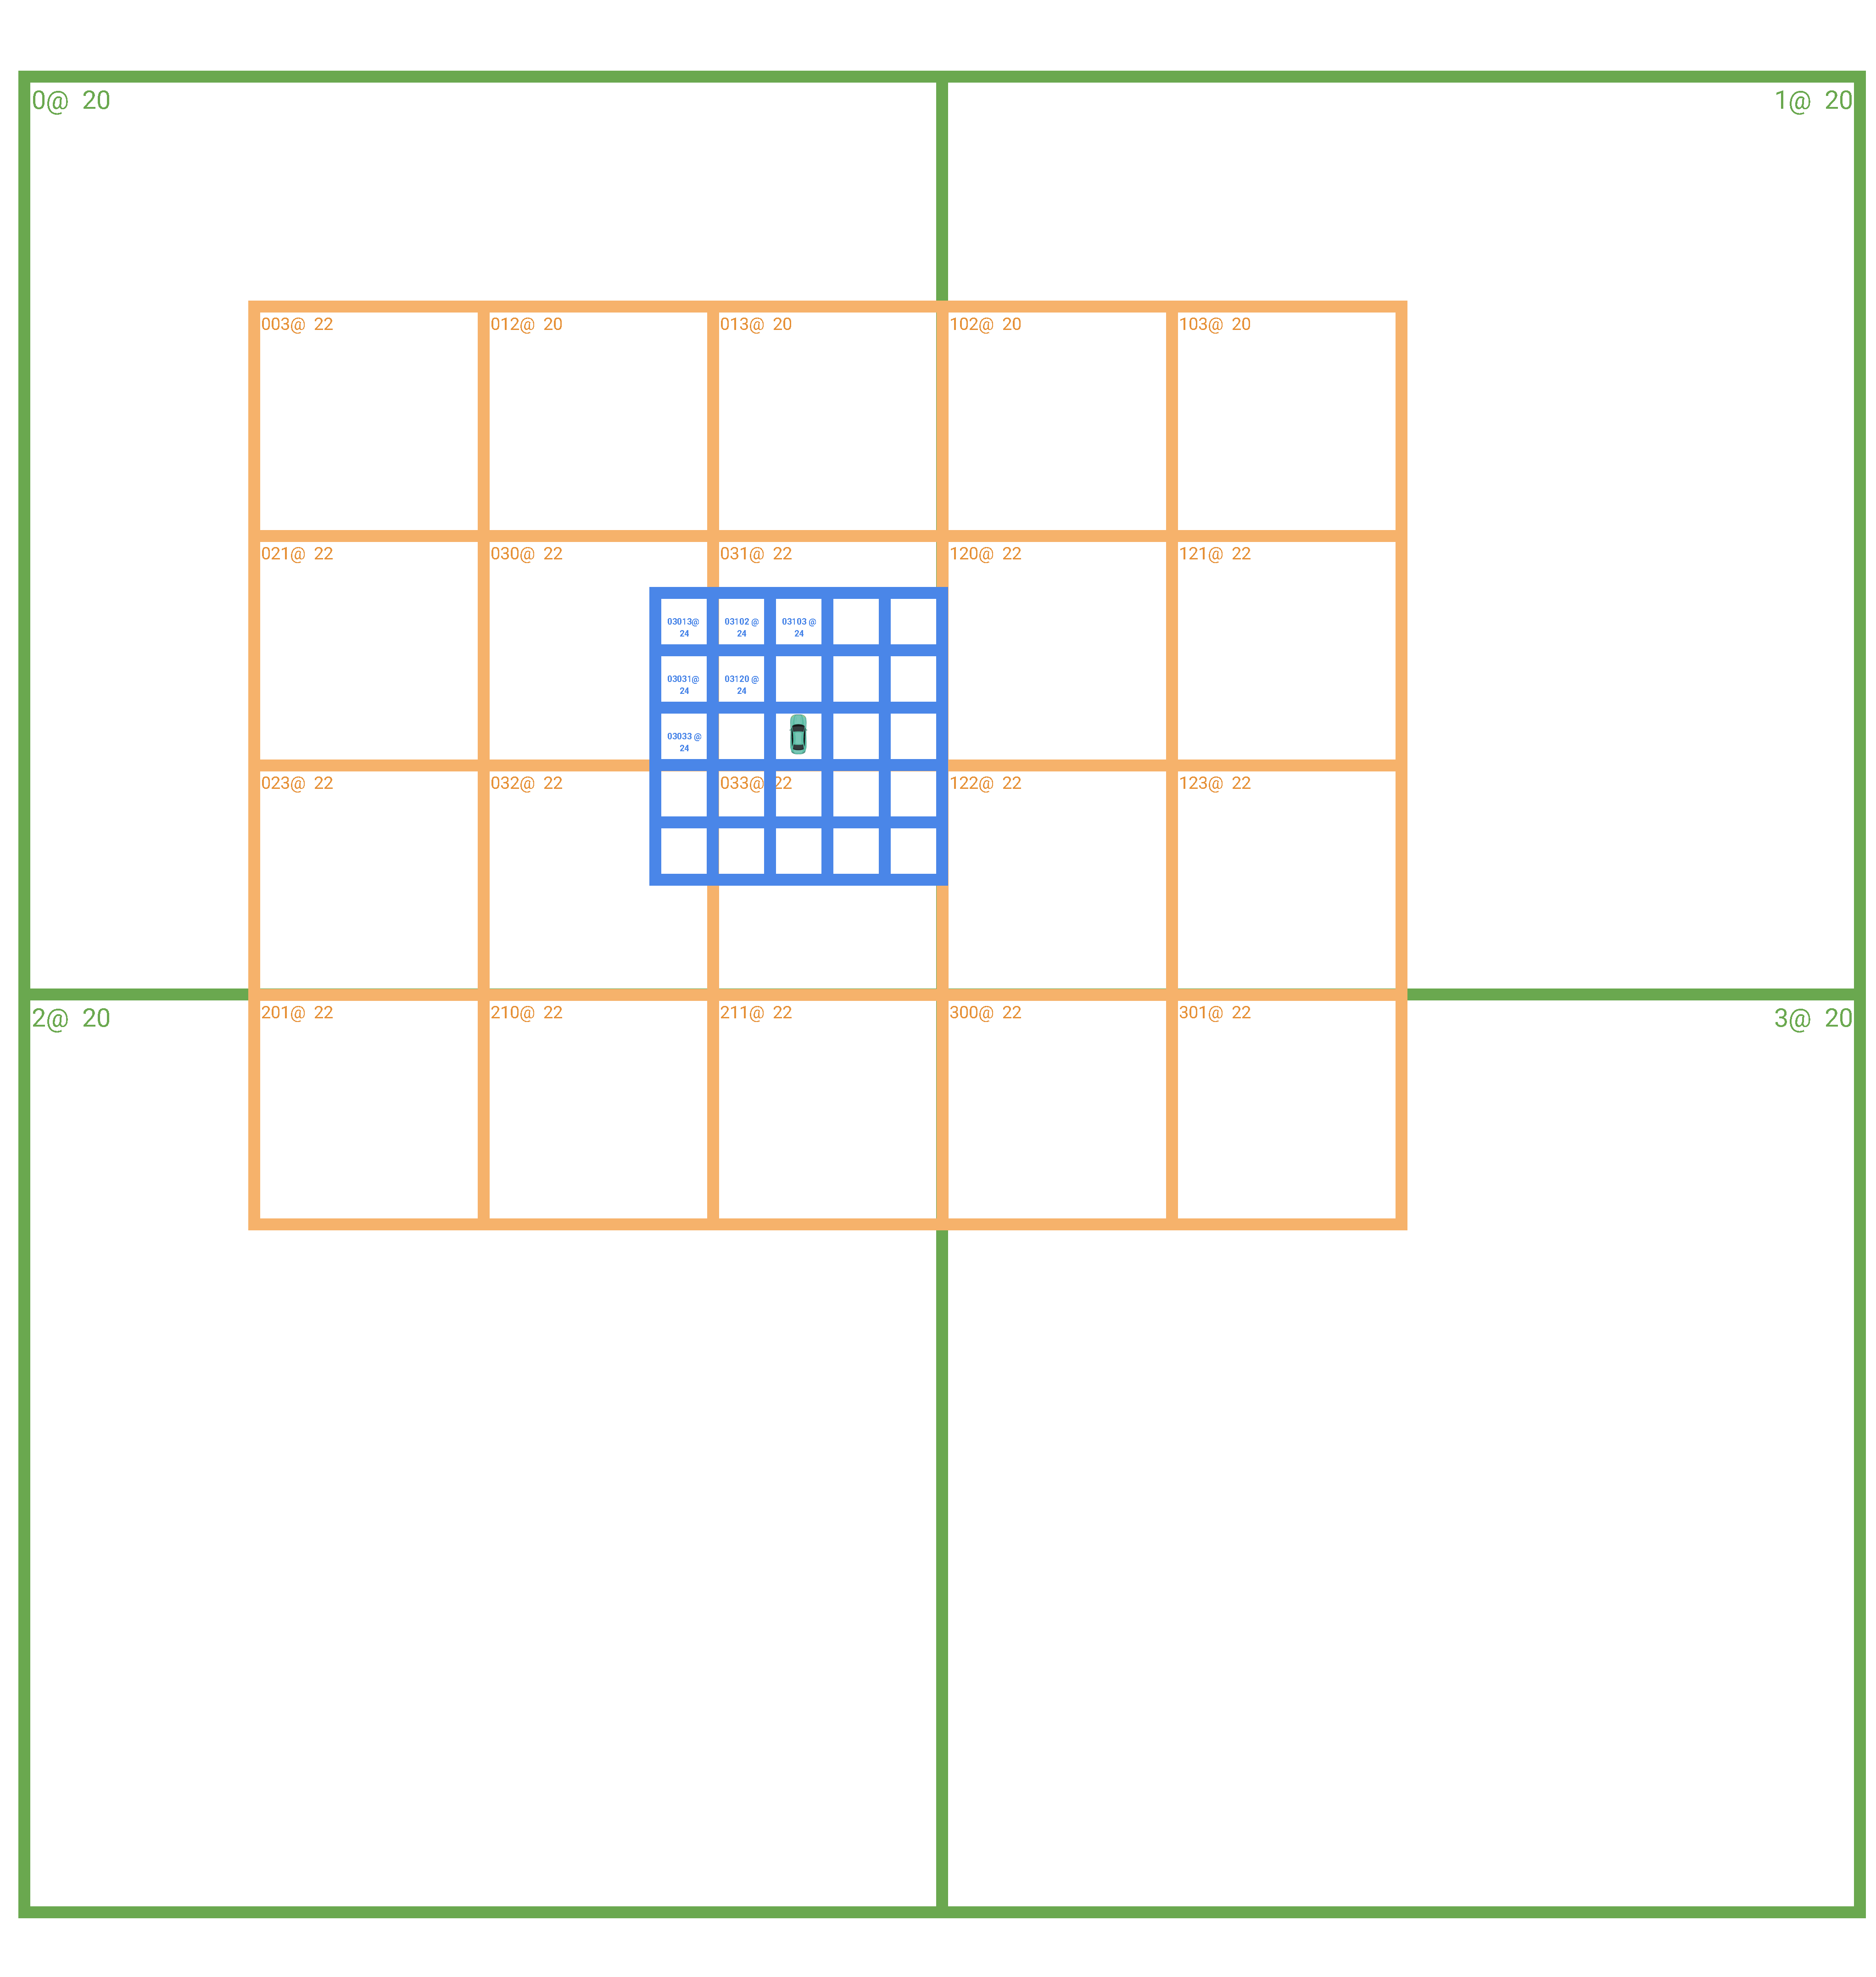
\includegraphics[width=0.9\linewidth]{98_images/geo_subscription_schema}
	\caption[Schematic Illustration of Geographical Sharding]{Schematic Illustration of Geographical Sharding \\ Blue cells (= type 1 tiles) are part of the vehicle's observed occupancy grid. \\ Orange cells (= type 2 tiles) are part of the vehicle's range of interest. \\ Green cells (=type 3 tiles) are subject to geo distribution.}
	\label{fig:geo_distribution_schema}
\end{figure}

\section{Evaluation}
\label{sec:appendix:texts:evaluation}

\subsection{Perception Evaluation Analyses}
\label{subsec:appendix:texts:evaluation:perception_relevant_analyses}
\begin{figure}[H]
	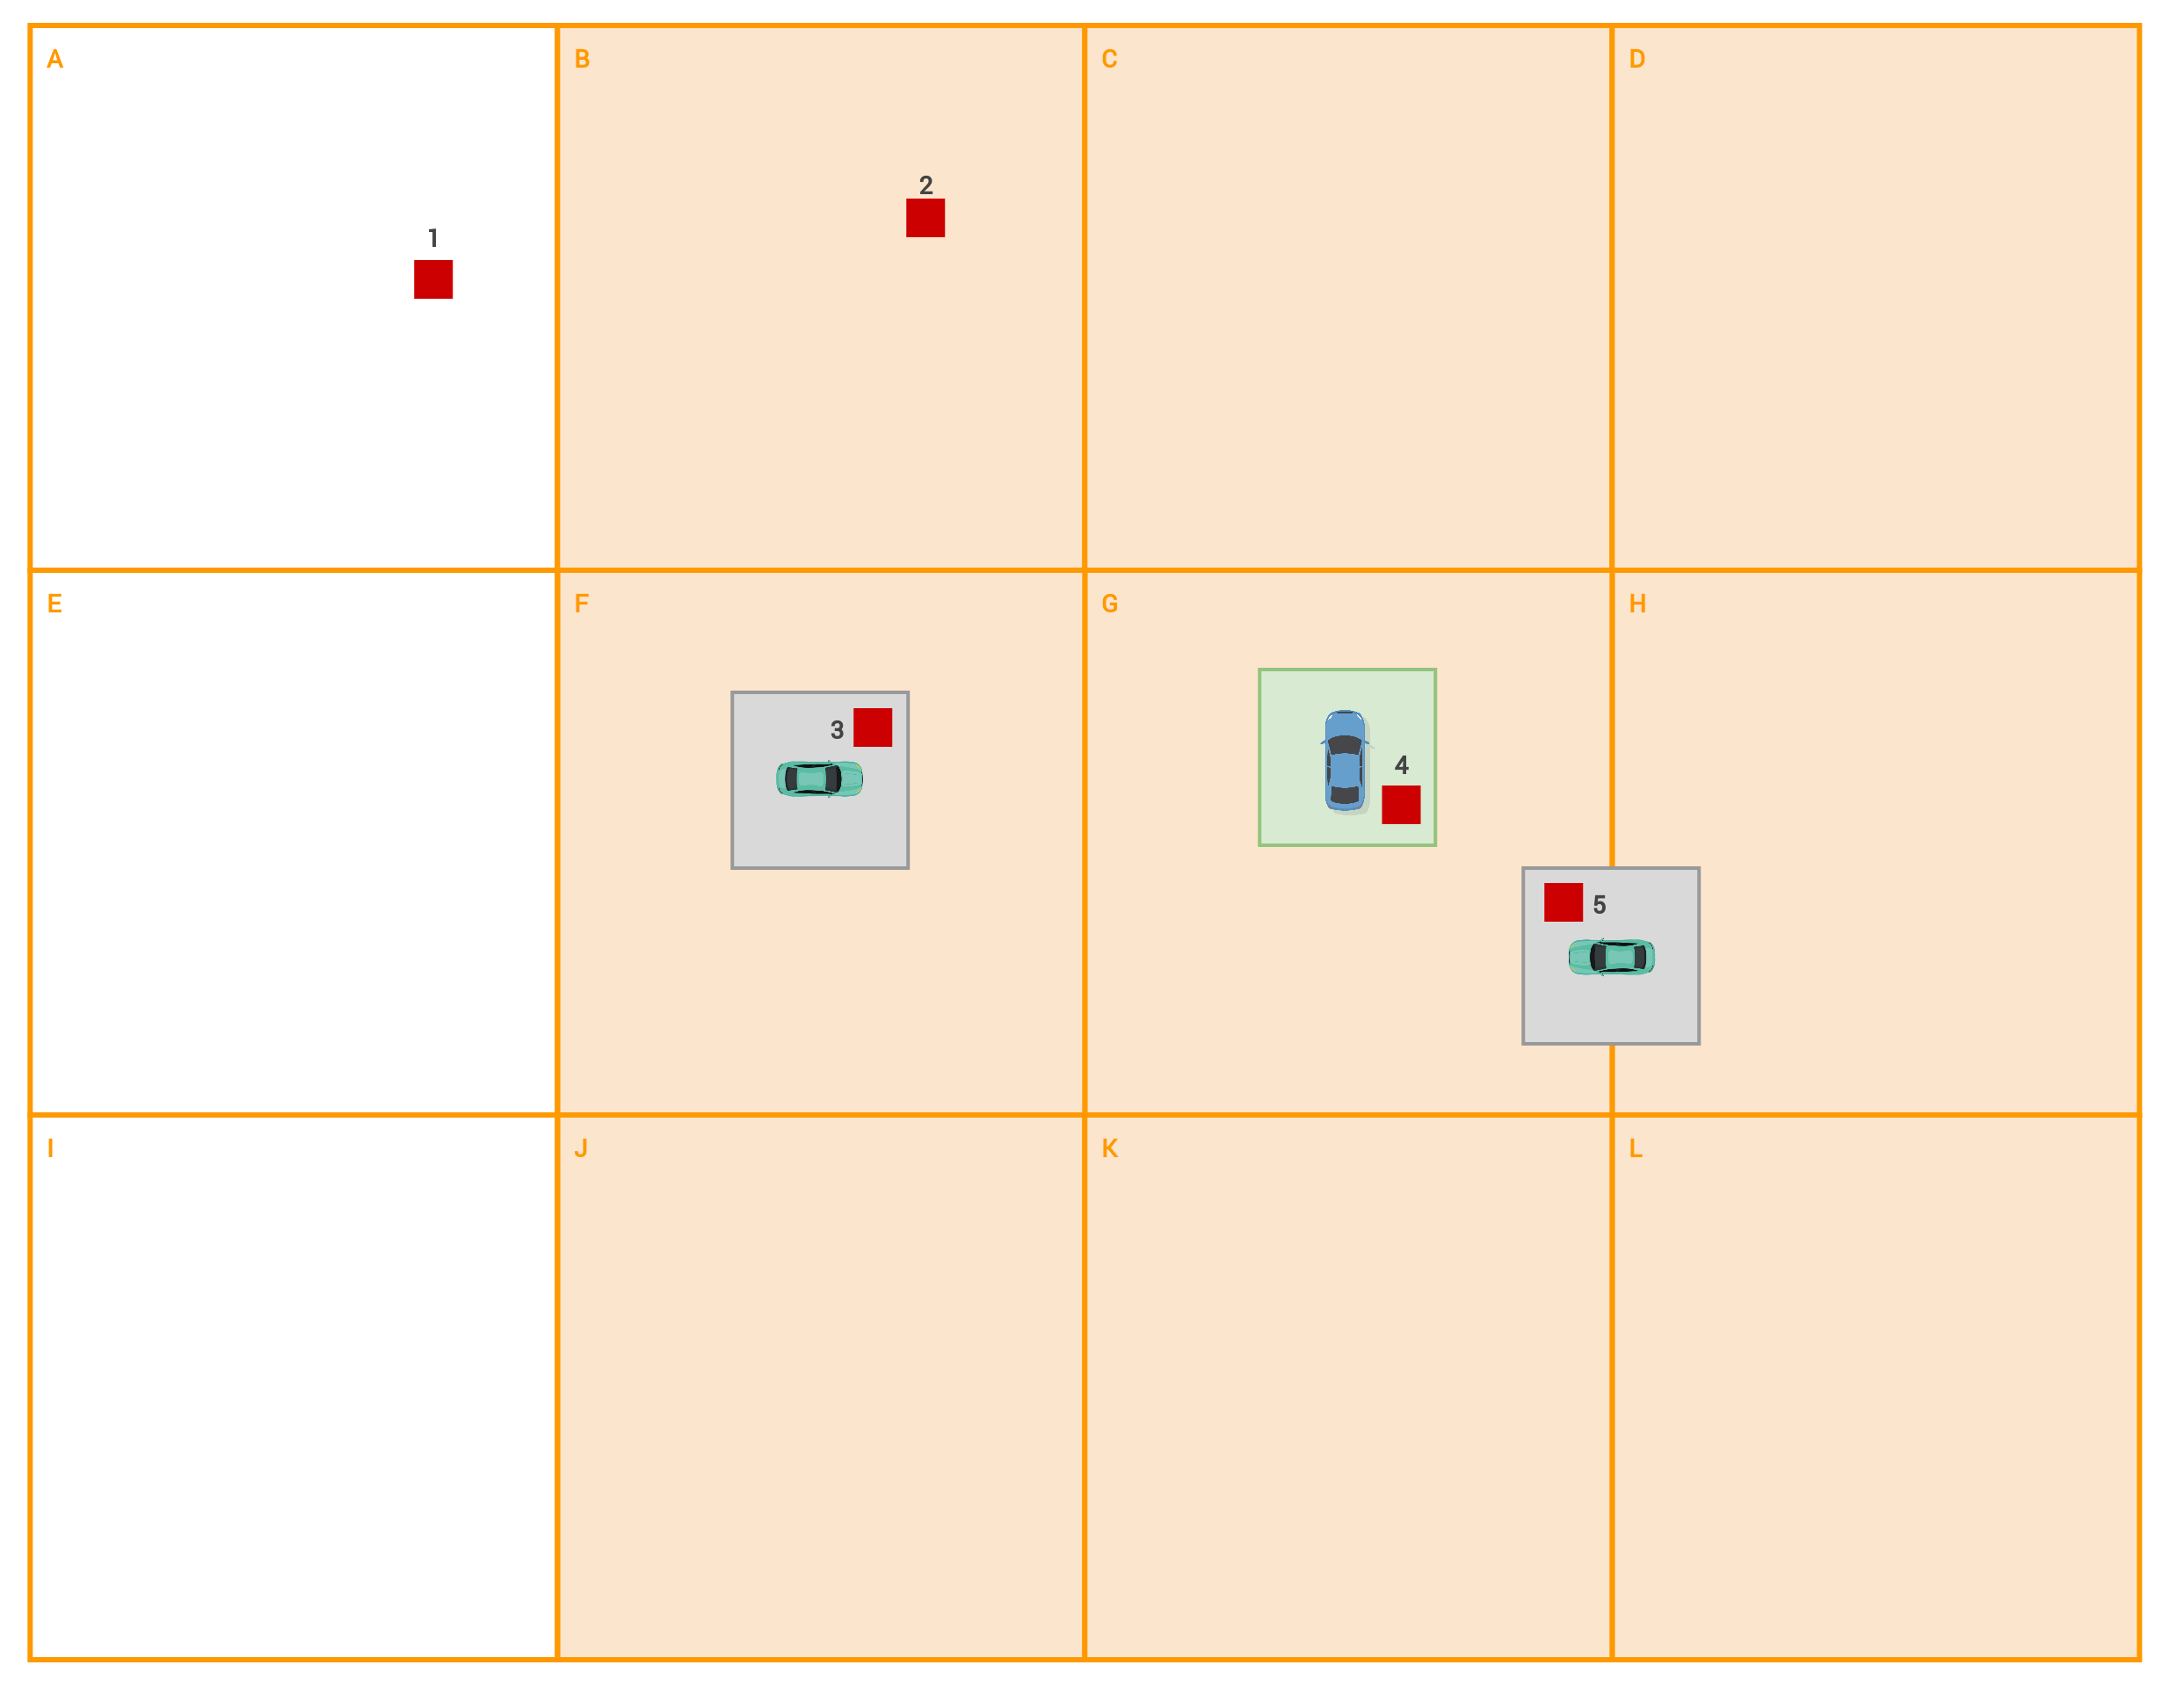
\includegraphics[width=1\linewidth]{98_images/grid_evaluation}
	\caption{Schematic Illustration of Evaluation-Relevant Cells}
	\label{fig:eval_relevant_cells}
	\medskip
	\small
	The blue vehicle is the ego vehicle in this example, while the green vehicles are other network participants. The orange type 2 cells are those, which the ego is currently subscribed to (i.e. its "'neighborhood"') for receiving observations from the fusion node. At the same time, they are the ones whose type 1 cells to include into the evaluation. Red rectangles depict obstacles and green or gray rectangles around vehicles show their respective observation range, i.e. local grid size.
	
	Obstacle 4 is within the ego's local observation range, while 2, 3 and 5 can only be recognized through CP with the help of other cars. Obstacle 1 is out of range for the ego, regardless of CP being turned on or off.
	
	Without CP, the ego can detect $\frac{1}{4}$ obstacles in potential range, while with CP it virtually detects $\frac{3}{4}$ of them.
\end{figure}

\chapter{Source Code}
\label{appendix:source_code}

\section{SQL Queries for Traffic Volume Estimation}
\label{sec:appendix:source_code:traffic_volume}

\subsection{Query: Geographic Area}
\inputminted[fontsize=\footnotesize]{sql}{97_listings/traffic_volume_1.sql}

\subsection{Query: Total Road Length}
\inputminted[fontsize=\footnotesize]{sql}{97_listings/traffic_volume_2.sql}

\subsection{Query: Average Number of Lanes}
\inputminted[fontsize=\footnotesize]{sql}{97_listings/traffic_volume_3.sql}

\section{Ray Casting Intersection Algorithm}
\label{sec:appendix:source_code:ray_casting_intersection_algorithm}
\inputminted[fontsize=\footnotesize]{c++}{97_listings/raycast.cu}

\chapter{Evaluation Results}
\section{Serialization Benchmark}
\label{sec:appendix:evaluation_results:serialization_benchmark}
\inputminted[fontsize=\footnotesize]{text}{97_listings/serialization_evaluation.txt}

\section{MQTT Broker Benchmark}
\label{sec:appendix:evaluation_results:mqtt_broker_benchmark}
\inputminted[fontsize=\footnotesize]{text}{97_listings/mqtt_bench.txt}